\documentclass{standalone}
\usepackage[T1]{fontenc}
\usepackage[latin2]{inputenc}
\usepackage[english]{babel}
\usepackage{tikz}
\usepackage{times}
\usetikzlibrary{calendar}

\usetikzlibrary{calc,through,backgrounds,positioning,fit}
\usetikzlibrary{shapes,arrows,shadows}

\begin{document}

	
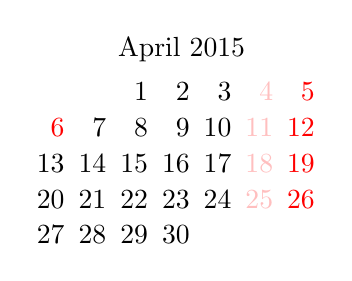
\begin{tikzpicture}
\calendar
[dates=2015-04-01 to 2015-04-last,week list,month label above centered,
month text=\textcolor{black}{\%mt} \%y-]
if (Sunday)            [red]
if (Saturday)            [pink]
if (equals=2015-04-06) [red]
;

\end{tikzpicture}
	
\end{document}